
\chapter{Search algorithm}
\label{search_algorithm}



Usually, Lagrangian frameworks involve the computation of the streamlines or projections. The computation of the streamlines is related to the material derivative and is part of the differentiation. The projections are related to the communication between the Lagrangian and Eulerian domains, and them belong to the numerical environment. Those task require the search of material points (streamlines) or nodes (projections) over the spatial discretization. This happens both in the fixed mesh PFEM-2 algorithm or in the mesh moving PFEM algorithm. As counterpart to the simplicity in the system computation provided by the Lagrangian algorithms, a search algorithm is required. In this appendix, the search algorithm used and implemented in the presented work is explained.

The cost of the search of intersections or point vicinity to objects is quadratic, all the objects have to be tested against all. However, this cost can be drastically reduced if the domain is subdivided in cells or bins, containing a few objects. 
The \emph{divide and conquer} strategy is based on the fact that the sum of the search of a few objects is smaller than the search of all the objects ($\sum\text{few}\cdot\text{few} \ll \sum\text{all}\cdot\text{all}$). The best method for dividing the objects in bins depends on the target geometries. Several trees can be defined using Axis-Aligned Bounding Boxes (AABB) \cite{samet1984} or Object-Oriented (OBB) \cite{gottschalk1996}. Figure \ref{tree_search} shows ans schematic of some tree partitions.

\begin{figure}[thb]
    \centering
    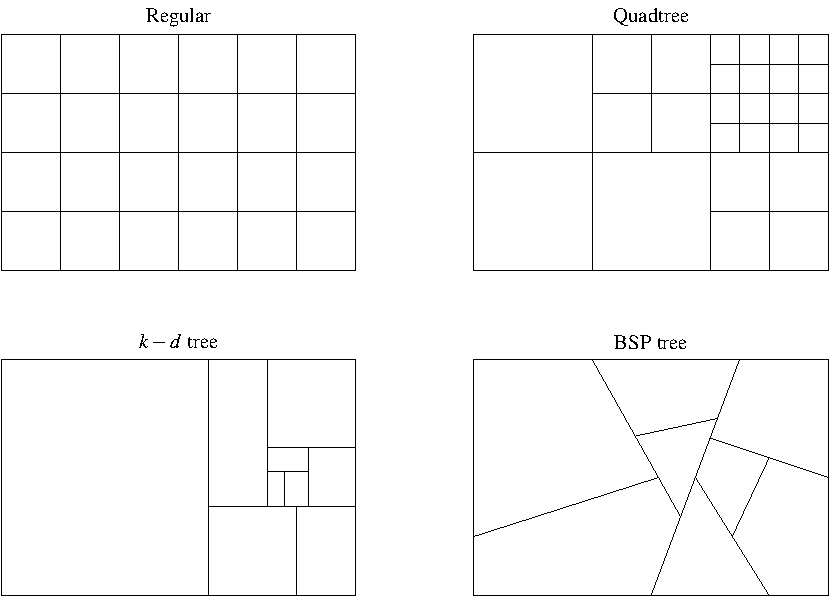
\includegraphics[width=.9\textwidth]{img/search/tree_search.pdf}
    \caption{Some common tree structures.}
    \label{tree_search}
\end{figure}

Since the computational domains are dense and we are not interested in the surface, but inside the body, an AABB structure will be employed (Fig. \ref{bins_search}).
Firstly, the main domain is partitioned using a dynamic bins structure, a detailed explanation can be found in \cite{samet1984}. In brief, the dynamic bins are a search structure where the cell size is higher than the characteristic element size, each cell contains a set of elements. Once the search structure is initialized, the location of a point is performed in two steps. The location on the cells, and the location on the candidate elements.

\begin{figure}[htb]
    \centering
    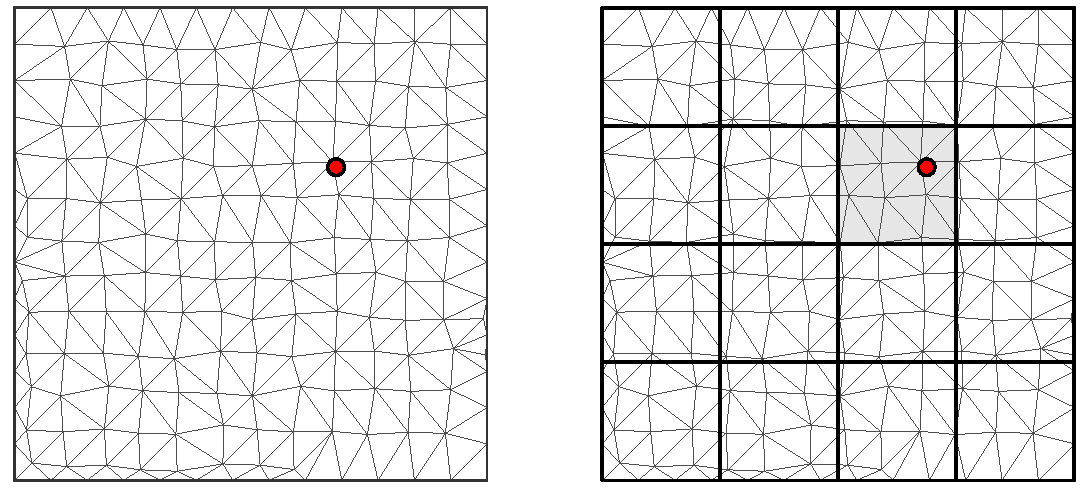
\includegraphics[width=.9\textwidth]{img/search/bins_search.pdf}
    \caption{Left: Mesh and entity to locate in the mesh. Right: Mesh and entity with the search structure (AABB)}
    \label{bins_search}
\end{figure}

Building the search structure has an initial cost, but is recovered during the search, specially when the mesh becomes larger. The definition of the cells is straightforward, while the main cost of the search structure building is the definition of the intersected elements against each cell. The element-cell intersections have been computed using the method described by Möller \cite{moller2004}, described below.

Once the bins structure is finalized, the search process is quite simple. Besides the fast process of locating a node, the location of multiple nodes can be executed in parallel. Both properties make this algorithm very efficient.

Hereafter, the most representative algorithms are described. Other direct intersection algorithms such as ray-triangle \cite{moller1997, jimenez2014} or triangle-triangle \cite{moller1997tritri} are used in this work, but for sake of brevity are not described here.




\section{Triangle vs aligned box intersection}

The full explanation of the algorithm can be found in \cite{moller2004}. Since this procedure is a generic tool for numerical methods, it has been applied for the shallow water, convection diffusion and Navier-Stokes equations. The generic 3D version is explained here, as well a the 2D particularization.

The derivation of this algorithm is based on the \emph{Separating Axis Theorem} \cite{gottschalk1996}. This theorem consists on looking fo a separating axis between the two objects. 
The algorithm looks for a separating axis along different directions. If a separating axis is found, the algorithm stops since there is not intersection. If all the tests pass, there is an intersection.
Figure \ref{triangle_aabb} shows the 13 possible directions where a separating axis can be found. To sum up, the directions are the three cartesian basis, $\mathbf{e}_i$, the normal vector $\mathbf{n}$ and the nine combinations of the triangle edges against the cartesian basis, $\mathbf{f}_j \times \mathbf{e}_i$.

\begin{figure}
    \centering
    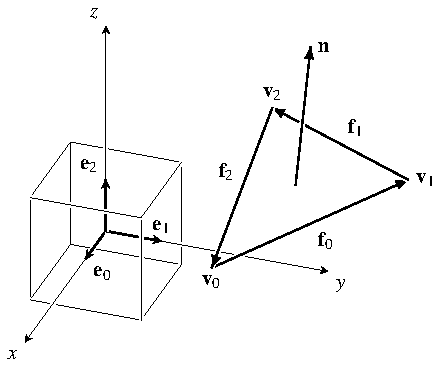
\includegraphics[width=.6\textwidth]{img/search/triangle_aabb.pdf}
    \caption{Notation for the triangle-AABB intersection test.}
    \label{triangle_aabb}
\end{figure}

According to Figure \ref{triangle_aabb}, the first operation consists on a translation in order to get the AABB in the origin of coordinates. The tests to evaluate are:


\begin{description}
    \item[Cartesian axis] (3 tests) The first set of tests involves the comparison of the AABB against the triangle AABB on the three directions $\mathbf{e}_i$. In pseudocode, the search of a separating axis is:
    \begin{verbatim}
for i = 0:2
    min, max = min_max(triangle_points)
    if (min > box_half_size or max < -box_half_size)
        return true
return false
    \end{verbatim}
    \item[Normal vector] (1 test) The second set of tests consists on the AABB-plane comparison. The plane containing the triangle is defined with the unit vector $\mathbf{n}$ and the distance to origin $d$. The test is performed in the same quadrant of $\mathbf{n}$ and is analogous to the previous one.
    \begin{verbatim}
for i = 0:2
    if (normal[i] > 0)
        box_half_size_proj += box_half_size[i] * normal[i]
    else
        box_half_size_proj -= box_half_size[i] * normal[i]
if (distance > box_half_size_proj)
    return true
return false
    \end{verbatim}
    \item[Edges] (9 tests) A test is performed for every axis $\mathbf{a}_{ij} = \mathbf{n}_i \times \mathbf{f}_j$. Each tests involves a projection of the triangle and the AABB. Fortunately, the expansion of the projections allow to make some simplifications. For the first projection we have:
    \begin{align*}
        p_0 &= \mathbf{a}_{00} \cdot \mathbf{v}_0 = (0, -f_{0z}, f_{0,y}) \cdot \mathbf{v}_0 = v_{0z}v_{1y} - v_{0y}v_{1z} \\
        p_1 &= \mathbf{a}_{00} \cdot \mathbf{v}_1 = (0, -f_{0z}, f_{0,y}) \cdot \mathbf{v}_1 = v_{0z}v_{1y} - v_{0y}v_{1z} = p_0 \\
        p_2 &= \mathbf{a}_{00} \cdot \mathbf{v}_2 = (0, -f_{0z}, f_{0,y}) \cdot \mathbf{v}_2 = (v_{1y} - v_{0y}) v_{2z} - (v_{1z} - v_{0z}) v_{2y}
    \end{align*}
    The fact that $p_0 = p_1$ makes easier the finding of the maximum and minimum of $p_0$, $p_1$ y $p_2$. Those are compared against the \emph{radius} of the box, which is the projection of the corner onto $\mathbf{a}_{00}$:
    \begin{align*}
        r = h_x |a_{00x}| + h_y |a_{00y}| + h_z |a_{00z}|
    \end{align*}
    Finally, finding a separating axis is:
    \begin{verbatim}
if (min(p0, p2) > r or max(p0, p2) < -r)
    return true
    \end{verbatim}
\end{description}
If the 13 tests return false, it means there is not a separating axis, thus, there is not intersection. Note that if one test returns true, the algorithm stops since there would not be a possible intersection.
In practice, the bullet 3 is evaluated at first, then bullet 1 and finally, bullet 2.



\subsection{2D particularization}

The two dimensional case is a simplification of the previous algorithm and some test can be omitted. Only five tests are needed:
\begin{description}
    \item[Cartesian axis] (2 tests) A separating axis is sought over $x$ and $y$.
    \item[Normal vector] (none) Is omitted.
    \item[Edges] (3 tests) Only the projections of the edges $\mathbf{f}_j$ against the edge $\mathbf{e}_z$ are relevant.
\end{description}



\section{Quadrilateral vs aligned box intersection}

The above algorithm is easily extrapolated to quadrilaterals. On the one hand, there is an extra edge test in the third bullet. On the other hand, looking for the minimum and maximum coordinate in the first bullet, involves more conditionals.

However, in practice, each quadrilateral is subdivided in two triangles and two comparisons are made. Even the number of tests is greater, this strategy allows to reduce code duplication and to make easier the code maintaining. This approach is done since we are not interested on the code optimization, but on the evaluation of the FEM. 



\section{Point intersection}

Determining if a point is inside a linear triangle or bilinear quadrilateral is a straightforward task. This procedure involves determining the local coordinates and verifying if all of them are between 0 and 1 for triangles, or between -1 and 1 for quadrilaterals.
An equivalent verification is expressed in terms of the shape functions $N$, this involves less conditionals than the previous case:
\begin{verbatim}
function is_inside
    for i = 1 : n_nodes
        if N(i) < 0
            return false
    return true
\end{verbatim}



